\section{Lecture 7}
\begin{itemize}
    \item Suppose we wish to rigorously prove an infinite limit.
    \begin{example}
        Prove $\displaystyle\lim_{x\to 0}\frac{1}{x^4}=\infty$.
        \begin{enumerate}
            \item Given: $M>0$
            \item It is required that $f(x)>M \implies \frac{1}{x^4} > M$
            \item when $0<|x-c|<\delta \implies 0<|x|<\delta$
            \item LHS of 2 is $|x|<\delta \implies \frac{1}{\delta^4} < \frac{1}{|x|^4}$. Therefore, the LHS of (2) is under $\delta$ control.
            \item Judgement: Try $\delta=\frac{1}{M^{1/4}}$. Therefore:
            \begin{equation}
                \text{LHS(2)} > \frac{1}{\delta^4} = M
                \label{eq:}
            \end{equation}
        \end{enumerate}
        Given $M>0$, choose $\delta=\frac{1}{M^{1/4}}$ then when $0<|x-0|<\delta$, we have $\frac{1}{x^4}>M$.
    \end{example}
    \item Instead of having to prove $\displaystyle \lim_{x\to c} f(x)=L$. What if we were given this statement? This leads to limit theorems:
    \begin{theorem}
        Given $\displaystyle\lim_{x\to c}f(x)=L$ and $\displaystyle\lim_{x\to c}g(x)=M$, then:
        \begin{equation}
            \lim_{x\to c}\left[f(x)+g(x)\right]=L+M
            \label{eq:}
        \end{equation}
        
    \end{theorem}
    \begin{prooof}
        \begin{enumerate}
            \item Given: $\epsilon>0$ is specified.
            \item It is required that:
            \begin{equation}
                |f(x)+g(x)-L-M| < \epsilon
                \label{eq:}
            \end{equation}
            \item ... when $0<|x-c|<\delta$
            \item The left hand side of (2) is:
            \begin{align}
                |(f(x)-L)+(g(x)-M)| \le |f(x)-L|+|g(x)-M|
                \label{eq:}
            \end{align}
            where we have applied the triangle inequality. Note that $\displaystyle \lim_{x\to c}f(x)=L$ is given here. As a result, we can now play the role of the $\epsilon$nemy and we can specify an number $\epsilon_f>0$ we want. Suppose we choose $\epsilon_f=\frac{\epsilon}{2}$. It is then guaranteed that some number $\delta_f>0$ exists for sure such that for all $0<|x-c|<\delta_f$ it can be proved that $|f(x)-L|<\epsilon_f=\frac{\epsilon}{2}$.
            \vspace{2mm}

            Similarly for $g(x)$ we can impose any $\epsilon_g>0$ we want, say $\epsilon_g = \epsilon/2$, and it is guaranteed that some $\delta_g>0$ exists such that for all $0<|x-c|<\delta_g$, then $|g(x)-M|<\epsilon_g=\epsilon/2$. Next, note that if $x$ is inside both $\delta_f$ and $\delta_g$ bands then:
            \begin{equation}
                \text{LHS (2)} < \epsilon/2 + \epsilon/2 = \epsilon   
                \label{eq:}
            \end{equation}
            as requested.
            \item Therefore, pick $\delta=\min\{\delta_f,\delta_g\}$.
        \end{enumerate}
        There are two possibilities, when $\delta_f>\delta_g$ or when $\delta_g>\delta_f$:
        \vspace{2mm}
        \begin{center}
            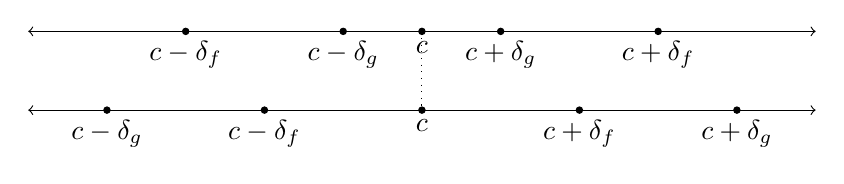
\begin{tikzpicture}
                \draw[<->] (-5,0) -- (5,0);
                \draw[fill=black] (0,0) circle (0.04) node[below] {$c$};
                \draw[fill=black] (-1,0) circle (0.04) node[below] {$c-\delta_g$};
                \draw[fill=black] (1,0) circle (0.04) node[below] {$c+\delta_g$};
                \draw[fill=black] (-3,0) circle (0.04) node[below] {$c-\delta_f$};
                \draw[fill=black] (3,0) circle (0.04) node[below] {$c+\delta_f$};

                \draw[<->] (-5,-1) -- (5,-1);
                \draw[fill=black] (0,-1) circle (0.04) node[below] {$c$};
                \draw[fill=black] (-2,-1) circle (0.04) node[below] {$c-\delta_f$};
                \draw[fill=black] (2,-1) circle (0.04) node[below] {$c+\delta_f$};
                \draw[fill=black] (-4,-1) circle (0.04) node[below] {$c-\delta_g$};
                \draw[fill=black] (4,-1) circle (0.04) node[below] {$c+\delta_g$};

                \draw[dotted] (0,0) -- (0,-1);
            \end{tikzpicture}
        \end{center}
        so when $0<|x-c|<\delta=\min\{\delta_g,\delta_f\}$, then $x$ satisfies both $0<|x-c|<\delta_f$ and $0<|x-c|<\delta_g$.
    \end{prooof}
    \begin{theorem}
        The product limit theorem says that $\displaystyle_{x\to c} f(x)g(x)=LM$ provided that both limits exist:
        \begin{equation}
            \lim_{x\to c}f(x)=L,\, \lim_{x\to c} g(x)=M
            \label{eq:}
        \end{equation}
        Do not use this theorem unless both limits exist!
    \end{theorem}
    \begin{theorem}
        The polynomial limit theorem says that $\displaystyle \lim_{x\to c} P_n(x) = P_n(c)$ given that $P_n(x)$ is a polynomial.
    \end{theorem}
    \begin{theorem}
        The rational function limit theorem:
        \begin{equation}
            \lim_{x\to c} \frac{f(x)}{g(x)} = \frac{1}{M},\, M\neq 0
            \label{eq:}
        \end{equation}
        and only applies when both limits exist.
    \end{theorem}
    \begin{theorem}
        The root limit theorem says that:
        \begin{equation}
            \lim_{x\to c} f(x)^{1/n} = L^{1/n}
            \label{eq:}
        \end{equation}
    \end{theorem}
    All of these limit theorems can be proven the same way as the additivity limit theorem, but proofs are not assigned. Therefore, the following is a completely rigorous proof.
    \begin{example}
        Determine $\displaystyle \lim_{x\to -2} \frac{x^2-x-6}{x^2-4}$.
        \vspace{2mm}

        We can write it as:
        \begin{align}
            \lim_{x\to -2} \frac{x^2-x-6}{x^2-4} &= \lim_{x\to -2} \frac{(x-3)\cancel{(x+2)}}{\cancel{(x+2)}(x-2)} & \text{(ok since }x+2\neq 0\text{ here.)} \\ 
            &= \frac{\displaystyle\lim_{x\to -2} (x-3)}{\displaystyle\lim_{x\to -2}(x-2)} & \text{(rational function LT)} \\ 
            &= \frac{-2-3}{-2-2} & \text{(polynomial LT)} \\ 
            &= \frac{5}{4}
        \end{align}
    \end{example}
    \item Another useful limit theorem is the sandwich limit theorem.
    \begin{theorem}
        Given:
        \begin{itemize}
            \item $\displaystyle \lim_{x\to c}f(x)=L$
            \item $\displaystyle \lim_{x\to c}h(x)=L$
            \item $f(x) \le g(x) \le h(x)$ near $c$, but not necessarily \textit{at} $c$.
        \end{itemize}
        Then:
        \begin{equation}
            \lim_{x\to c}g(x)=L
            \label{eq:}
        \end{equation}
    \end{theorem}
    \begin{example}
        Determine $\displaystyle \lim_{x\to 0} x^2\cos^2\left(\frac{1}{x^2}\right)$
        \vspace{2mm}

        We might naively try to apply the product LT, but $\displaystyle \lim_{x\to 0}\cos^2\left(\frac{1}{x^2}\right)$ is not defined! Instead, we can apply the sandwich LT. Note that:
        \begin{align}
            0 \le \cos^2\left(\frac{1}{x^2}\right) \le 1
        \end{align}
        provided that $x\neq 0$. We can multiply both sides by $x^2$ since it is a positive quantity, then:
        \begin{equation}
            0 \le x^2\cos^2\left(\frac{1}{x^2}\right)\le x^2
            \label{eq:}
        \end{equation}
        We can rigorously find the limits of the two extremes of the inequality. We can define:
        \begin{align}
            f(x) \equiv 0 \\ 
            g(x) \equiv x^2\cos^2\left(\frac{1}{x^2}\right) \\ 
            h(x) \equiv x^2
        \end{align}
        Note that:
        \begin{align}
            \lim_{x\to 0}f(x)&=0 \\ 
            \lim_{x\to 0}h(x)&=0
            \label{eq:}
        \end{align}
        so by the sandwhich limit theorem:
        \begin{equation}
            \lim_{x\to 0} g(x) = \lim_{x\to 0} x^2\cos^2\left(\frac{1}{x^2}\right)=0.
            \label{eq:}
        \end{equation}
    \end{example}
\end{itemize}